\documentclass[a4paper,10pt]{report}  % >>>>>>> COMPILATION LuaLatex <<<<<<<
%********************************************************
%**************** Chargement des paquets ****************
%********************************************************
%-------------------------------------%******************
%-------------------------------------%   MISE EN PAGE  *
%-------------------------------------%******************
\usepackage[a4paper, left=2.5cm, width=16cm, height=25.4cm, includehead, includefoot, headheight=13.6pt]{geometry}
\usepackage{multicol}                 % Ecrire en colones \begin{multicols}{2} \end{multicols}
\usepackage[explicit,clearempty]{titlesec}	% Titres personalisables
\usepackage[hidelinks]{hyperref}      % Lien vers les chapitres en table de matières
  \hypersetup{pdfencoding=unicode}
\usepackage{fancyhdr}		          % En-tête et pied de page
\usepackage{enumitem}                 % Enumérations
\usepackage{tcolorbox}                % Boîtes en couleur avex titre ...
  \tcbuselibrary{minted,skins,theorems}
  \tcbset{listing engine=minted}
%\usepackage{nameref}
%-------------------------------------%******************
%-------------------------------------%    CARACTERES   * 
%-------------------------------------%******************
\usepackage{fontspec}   
  \setmonofont[Scale=MatchLowercase,BoldFont={Inconsolatazi4 Bold}]{Inconsolatazi4}
  \newfontfamily\inconsola{Inconsolatazi4}
  \newfontfamily\greekfont[Script=Greek, Scale=MatchUppercase, Ligatures=TeX]{Arial}
  \newcommand{\textgreek}[1]{\bgroup\greekfont#1\egroup}
\usepackage{polyglossia}
  \setmainlanguage{french}
  \setotherlanguage{english}
\usepackage{pifont}                   % Pour les \ding{} caractères images
%-------------------------------------%******************
%-------------------------------------%  MATHEMATIQUES  *
%-------------------------------------%******************
\usepackage{amssymb,                  % Symboles mathématiques
            amsthm}                   % Personalisation des théorèmes
\usepackage[np]{numprint}	          % Pour l'écriture des nombres \np{3250.58}
%-------------------------------------%******************
%-------------------------------------%    GRAPHIQUES   *
%-------------------------------------%******************
\usepackage{pgf,tikz}			 	  % Dessinner avec tikz
\usepackage{graphicx}	              % Inclusion d'images


%********************************************************
%************ PERSONALISATIONS ET RACOURCIS *************
%********************************************************
%--------------------------------------------------------
%---------------- Formatage des entêtes -----------------
\pagestyle{fancy}
\fancyhead{}\lhead{\leftmark\rightmark}\renewcommand{\headrulewidth}{0.1pt}\rhead{\thepage}
\lfoot[]{}\cfoot{}\rfoot[]{}
%--------------------------------------------------------
%--------------- Formatage des chapitres ----------------
\newcommand\rubrique{rubrique}
\renewcommand{\chaptermark}[1]{\markboth{\rubrique{} > #1 - }{}}
\titleformat{\chapter}[display]     % Formatage des titres de chapitre
    {\LARGE \bfseries}
    {\begin{tikzpicture}
    \node[draw,text width = \textwidth-\pgflinewidth-10pt,inner sep = 5pt,align = center](Ch){\strut\begin{minipage}{0.66\textwidth}\centering#1\end{minipage}};
    \node[right=1em,fill=white,inner sep=0]at(Ch.north west){\small\sc \rubrique};
    %\node[left=0.2em,fill=black!5,inner sep=4pt]at(Ch.east){\Huge \thechapter};
    \end{tikzpicture}}
    {0pt}
    {\tiny}[\setcounter{exo}{0}]
\titlespacing*{\chapter}{0cm}{-1.5cm}{-1em}[0pt]

%--------------------------------------------------------
%--------------- Formatage des sections -----------------
\renewcommand{\thesection}{\arabic{section}.~}
\renewcommand{\sectionmark}[1]{\markright{#1}}
\titleformat{\section}  
  {\gdef\sectionlabel{}\Large\bfseries}
  {\gdef\sectionlabel{\thesection }}{0pt}
  {#1}
\titlespacing*{\section}{0pt}{\baselineskip}{0.5\baselineskip}
%--------------------------------------------------------
%------------ Formatage des sous-sections ---------------
\renewcommand{\thesubsection}{\alph{subsection}.}
\titleformat{\subsection}  
  {\gdef\subsectionlabel{}\large\bfseries}
  {\gdef\subsectionlabel{\thesubsection }}{0pt}
  {#1}
\titlespacing*{\subsection}{0.33\parindent}{0.5\baselineskip}{0em}
%--------------------------------------------------------
%--------------- Formatage des listes -------------------
\setlist[itemize,1]{label=$\star$,nosep}
\setlist[itemize,2]{label=$-$}
\setlist[enumerate,1]{leftmargin=0.66\leftmargin,nosep}
\renewcommand{\labelenumi}{\textbf{\theenumi.}}
\setlist[enumerate,2]{leftmargin=0.66\leftmargin,label=\textbf{\alph*.},nosep}
%--------------------------------------------------------
%------- espacement verticaux d'un multicols ------------
\multicolsep\itemsep
%--------------------------------------------------------
%---------------------- Exercices -----------------------
\newtcbox{\titrexo}{on line,colback=black!5!white, colframe=black!75!black, 
size=small, left = 3mm, enhanced, overlay={\begin{tcbclipinterior}\fill[red!20!black!20!white] (frame.south west)rectangle ([xshift=3mm]frame.north west)node[midway, rotate = 90, color = black, xscale=0.75]{\bfseries\tiny Exo};\end{tcbclipinterior}}}
\newtheoremstyle{exo}{0.25\baselineskip}{0}{}{0pt}{}{}{ }{\titrexo{\bfseries#2#3}}  
\theoremstyle{exo}
\newtheorem{exo}{}
%-------------------------------------------------------%
%-- Commande pour une suite de points ------------------%
\newcommand\pointsuite[1]{\leavevmode\hbox to#1{\dotfill}} % \pointsuite{1.5cm} par exemple

%--------------------------------
%- Définitions-------------------
%--------------------------------
\newtcbtheorem[number within=chapter]{définition}{Définition}%
{colback=green!5!white,
colframe=green!75!black,
fonttitle=\bfseries,colbacktitle=green!65!black,
enhanced,separator sign dash,
attach boxed title to top left={xshift=2mm,yshift=-2mm}}{def}
%--------------------------------
%- Exemples----------------------
%--------------------------------
\newtcbtheorem[number within=chapter]{exemple}{Exemple}%
{colback=black!5!white,
colframe=black!25!white,leftrule=3mm, rightrule=0mm, bottomrule=0mm, toprule=0mm,
boxsep=0mm,boxed title style={empty,size=minimal},
fonttitle=\bfseries,coltitle=black,
enhanced,
separator sign dash,
attach boxed title to top left,
left=2mm,right=0mm}{def}

%********************************************************
%--------------------- Informatique ---------------------
%--------------------------------------------------------
%--------------------- Python ---------------------
\newtcblisting{python}[1][]{
  colback=blue!5!white, colframe=blue!75!black,
  listing only,
  minted language=python3,
  minted options={linenos=true,numbersep=3mm,texcl=true,#1},
  left=5mm,enhanced,
  overlay={\begin{tcbclipinterior}\fill[red!20!blue!20!white] (frame.south west)rectangle ([xshift=5mm]frame.north west);\end{tcbclipinterior}}
}
\newtcblisting{console}[1][]{
  colback=blue!5!white, colframe=blue!75!black,
  listing only,
  minted language=python3,
  minted options={texcl=true,#1},
  left=0mm,
  enhanced
}
%--------------------- Algorithmes ---------------------
\usepackage[french,boxed,vlined,longend]{algorithm2e} 
\DontPrintSemicolon                            % n'affiche pas les << ; >> de fin d'instruction
\SetKw{Retour}{renvoyer}                       % Redéfinition possible de tous les mots clefs
\SetKwProg{Fct}{fonction}{}{fin fonction}      % Définition possible d'autres environnements
\newcommand{\nonl}{\renewcommand{\nl}{\let\nl\oldnl}} % Retire la numérotation d'une ligne

%********************************************************
%---------------------- Correction ----------------------
%--------------------------------------------------------
\newcommand{\prof}[1]{\begin{tikzpicture}[overlay,baseline=(T.base)]\node[right, inner sep=0](T){\raisebox{2pt}{\color{blue!70!black}#1}};\end{tikzpicture}}
%\renewcommand\prof[1]{}

\begin{document}
\renewcommand\rubrique{Algorithmique}
\chapter{Recherche textuelle}

\section{Motivation}

\subsection{Nombres univers}

Il existe des nombres réels dont l'écriture des décimales renferme l'écriture de tous les entiers naturels, donc toutes les données informatiques imaginables : de véritables tours de Babel. Un tel nombre est appelé << nombre univers >>. On peut, par exemple, en construire un artificiellement en juxtaposant simplement l'écriture de tous les entiers.

\begin{exemple*}{Nombre de Champernowne}
David Gawen Champernowne (1912-2000) est un statisticien anglais dont les travaux sur les << nombres normaux >> ont été publiés en 1933. Il y présente en particulier ce nombre :

\np{0.1234567891011121314151617181920212223242526272829303132333435363738394041}...
\end{exemple*}

Parmi les nombreuses conjectures sur le nombre $\pi$, on pense qu'il est un nombre univers.

\begin{exemple*}{$\pi$ serait un nombre univers}
Fabien Olicard, est un mentaliste contemporain, auteur de livres, de spectacles et Youtubeur. Dans un de ses spectacles, il propose de retrouver quelles décimales de $\pi$ correspondent à la date d'anniversaire d'un spectateur...

\np{3.14159265358979323846264338327950288419716939937510582097494459}{\bfseries2}\,{\bfseries307}\,\np{816}\,\np{4}...

Quelqu'un né le 23/07 a sa date d'anniversaire entre les 63$^\text{e}$ et 66$^\text{e}$ décimales de $\pi$. 
\end{exemple*}

\subsection{Bio-informatique}
Le bio-informaticien / la bio-informaticienne fait le pont entre la biologie et l'informatique. Il/elle conçoit et met en œuvre des programmes informatiques pour aider les biologistes à mieux comprendre le monde du vivant. 

\begin{multicols}{2}
Par exemple l'information génétique est portée par les molécules d'ADN, qui sont, entre autres, composées de bases azotées : {\bfseries A}dénine, {\bfseries T}hymine, {\bfseries G}uanine et {\bfseries C}ytosine. Ces informations sont donc souvent représentées par une longue chaine composée des caractères A, T, G et C. 

C'est la succession précise et l'enchainement de groupes de trois bases qui sont susceptibles d'avoir du sens pour le << code génétique >>.

\begin{center}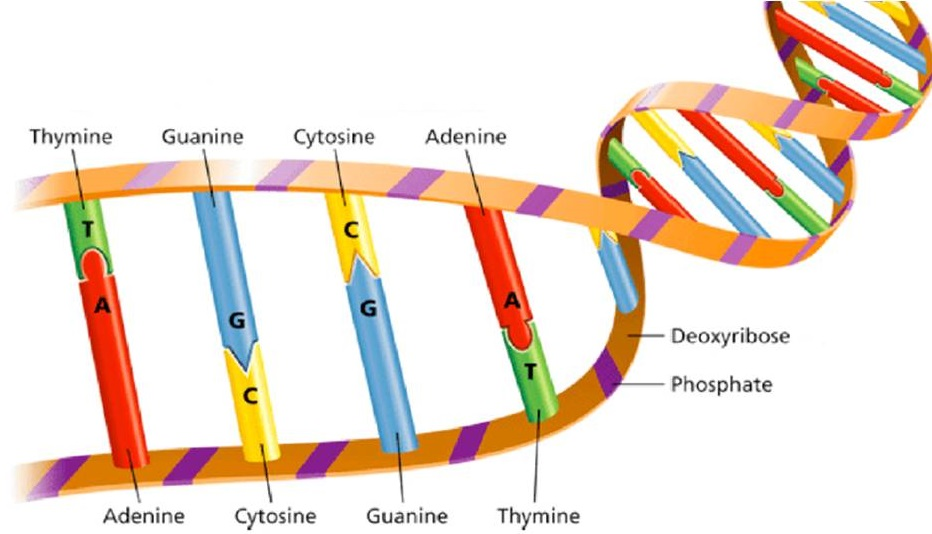
\includegraphics[width=0.85\linewidth]{adnb.jpg}\end{center}
\end{multicols}

\begin{exemple*}{Code génétique (\href{http://barraud.pythonanywhere.com/app/recherche-naive}{http://barraud.pythonanywhere.com/app/recherche-naive})}
Retrouve-t-on la séquence \texttt{CAGGAG} ci-dessous ? Combien de fois ? Où ? 

\ttfamily
CAATGTCTGCACCATGACGCCGGCATCTGCGAAGGCAGGAGCATGACCATGATTTCGAACCTACTAGTGGGTCTCTTAGGCCGAGCGGTTCC

GAGAGATAGTGAAAGATGGCTGGGCTGTGAAGGGAAGGAGTCGTGAAAGCGCGAACACGAGTGTGCGCAAGCGCAGCGCCTTAGTATGCTCC

AGTGTAGAAGCTCCGGCGTCCCGTCTAACCGTACGCTGTCCCCGGTACATGGAGCTAATAGGCTTTACTGCCCAATATGACCCCGCGCCGCG
\end{exemple*}

\subsection{Pratiques informatiques courantes}

Quand on fait une recherche d'information à travers Internet, on utilise un moteur de recherche, mais on peut parfois obtenir une page très longue ou un document de référence - une notice - de plusieurs dizaines de pages en \texttt{PDF}, ou sous un autre format. Il est alors utile de pouvoir faire une recherche de mots-clefs dans ces pages. Le raccourci clavier est généralement [Ctrl]+[F] (F pour \textit{find}).

Du côté du programmeur, qui définit des variables et des fonctions dont il a besoin, certains éditeurs de textes mettent même directement en surbrillance les occurrences d'un mot sélectionné...

\section{Algorithme << naïf >>}

\begin{exo}Proposer un algorithme permettant de répondre au dernier exemple (de recherche génétique).
\end{exo}

\subsection{Algorithme de la fenêtre glissante}



À chaque étape, on ne considère qu'une partie du texte, de la taille du motif recherché, comme si on le regardait à travers une fenêtre. On fait alors << glisser >> cette fenêtre d'une lettre vers la droite.

\noindent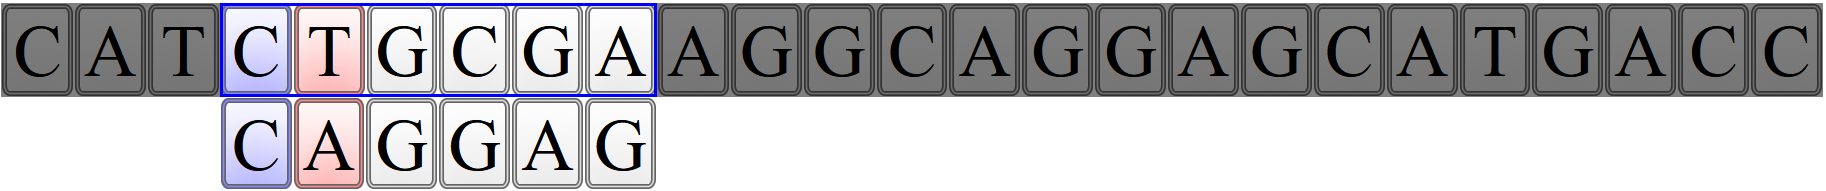
\includegraphics[width=\textwidth]{fenetreglissante.png}

(\href{http://barraud.pythonanywhere.com/app/Boyer-Moore}{http://barraud.pythonanywhere.com/app/Boyer-Moore}) On en déduit l'algorithme suivant :
%
%\begin{algorithm}[H]
%\Fct{recherche\_naive(texte,motif)}{
%  $\text{position} \leftarrow [~]$\;
%  \Pour{chaque position possible du motif dans le texte de gauche à droite}{
%      En partant de la lettre de gauche : \;
%      \Tq{la lettre du motif correspond et il en reste à tester}
%      {   Passer à la suivante \;   }
%      \Si{toutes les lettres sont identiques}{Ajoute $i$ à position\;}
%  }
%  \Retour{position}
%}
%\end{algorithm}
%
%Soit, en précisant les indices :

\begin{algorithm}[H]
\Fct{recherche(texte,motif)}{
  $\text{position} \leftarrow  $ liste vide\;
  \Pour{$i$ {\color{black}\bfseries\textrm allant de}  $0$ {\color{black}\bfseries\textrm à} $\text{taille}(\text{texte})-\text{taille}(\text{motif})$}{
      $j \leftarrow 0$\;      
      \Tq{$j<\text{taille}(\text{motif})$ et $\text{texte}[i+j]=\text{motif}[j]$}
      {   $j \leftarrow j+1$\;   }
      \Si{$j=\text{taille}(\text{motif})$}{Ajoute $i$ à position\;}
  }
  \Retour{position}
}
\end{algorithm}

\begin{exo} Programmation


\begin{enumerate}
    \item Programmer en Python l'algorithme précédent et vérifier les résultats suivants :
\begin{console}            
>>> recherche('CATCTGCGAAGGCAGGAGCATGACC', 'CAGGAG')
[12]                              
>>> recherche('CATCTGCGAAGGCAGGAGCATGACC', 'ATGACC')
[19]                          
>>> recherche('CATCTGCGAAGGCAGGAGCATGACC', 'GG')
[11, 14]
\end{console}
    \item Récupérer le fichier \texttt{pi1000000.txt} qui contient le premier million des décimales de $\pi$ et compléter le programme précédent par l'en-tête :
    
\begin{python}
pi = ""
with open('pi1000000.txt', encoding='utf8') as decimale:
    for line in decimale:
        pi = pi + line[:-1]
\end{python}

On code les jours de l'année sous la forme \texttt{jjmm}. Par exemple, le $1^\text{er}$ avril est noté \texttt{0104}.

\begin{enumerate}
    \item À quelle décimale de $\pi$ trouve-t-on le $1^\text{er}$ avril pour la première fois ?
    \item À quelle décimale de $\pi$ trouve-t-on votre jour d'anniversaire pour la première fois ?
    \item Si on ajoute les deux derniers chiffres de l'année, le $1^\text{er}$ avril 2021 se note \texttt{010421}. Vérifier que cette date apparait exactement une fois parmi le premier million de décimales de $\pi$. Qu'en est-il de votre jour de naissance ?
\end{enumerate} 
\end{enumerate}
\end{exo}

\subsection{Idées d'améliorations}

On considère la situation de départ suivante :

\noindent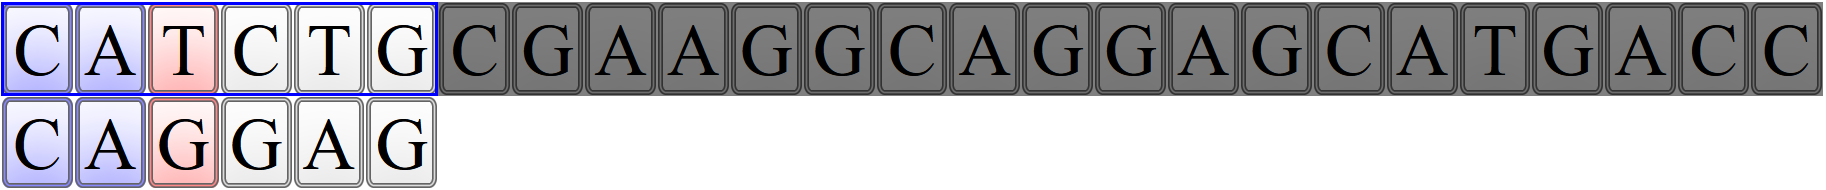
\includegraphics[width=\textwidth]{fenetreglissante0.png}

Après 3 comparaisons on obtient une non-concordance et on avance donc la fenêtre d'une lettre...

Pourrait-on, sans risque, avancer davantage la fenêtre ? (justifier)

\medskip\prof{On peut avancer de 3 car T n'est pas du tout dans le motif.}\dotfill

Dans la situation précédente, on a utilisé l'information du << mauvais caractère >>.

L'autre idée est alors naturellement : peut-on utiliser les informations des bons caractères ?

Au premier abord, la réponse est non. Si on considère que le premier caractère est bon :  dès qu'on fait glisser la fenêtre vers la droite, ce caractère n'a plus aucune importance pour les prochaines comparaisons. Deux solutions sont possibles :
\begin{itemize}
    \item Commencer la recherche par la fin du texte et faire glisser la fenêtre vers la gauche.
    \item Commencer les comparaisons par la fin du motif.
\end{itemize}
Si on veut pouvoir modifier l'algorithme pour qu'il ne renvoie la position ou l'existence que de la première occurrence du motif dans le texte, la première solution n'est pas bonne. Pour la suite, on va donc faire les comparaisons par la droite.

\begin{exo}
Compléter par le nombre de décalage :

\noindent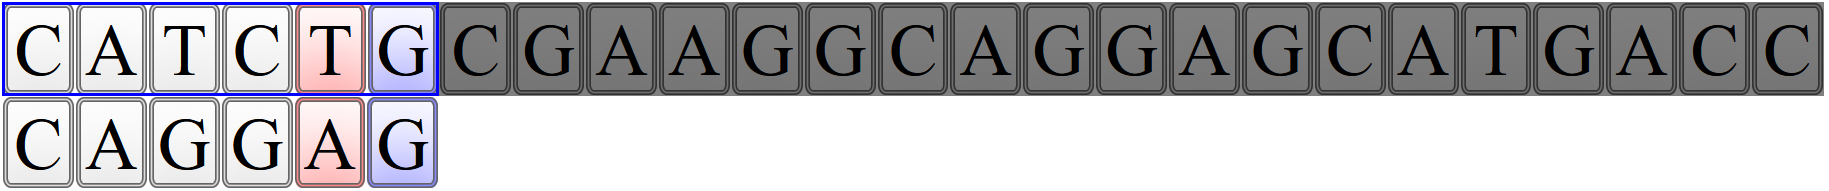
\includegraphics[width=\textwidth]{fenetreglissante1.png}

Utilisation du mauvais caractère : on avance de \prof{5}\pointsuite{1cm}

\medskip
\noindent
\includegraphics[width=\textwidth]{fenetreglissante2.png}

Utilisation du bon suffixe : on avance de \prof{3}\pointsuite{1cm}
\end{exo}

\section{Utilisation du mauvais caractère} 

\subsection{Pré-traitement}

Si le mauvais caractère n'est pas dans le motif, on peut avancer la fenêtre jusqu'à le dépasser.

On peut également tenir compte d'un mauvais caractère présent dans le motif. Par exemple :

\noindent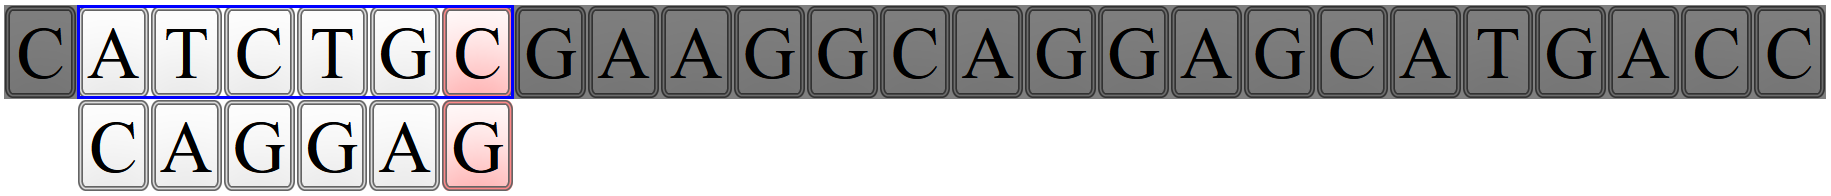
\includegraphics[width=\textwidth]{fenetreglissante3.png}

On sait où le mauvais caractère apparait dans le motif. On peut déplacer la fenêtre en conséquence :

\noindent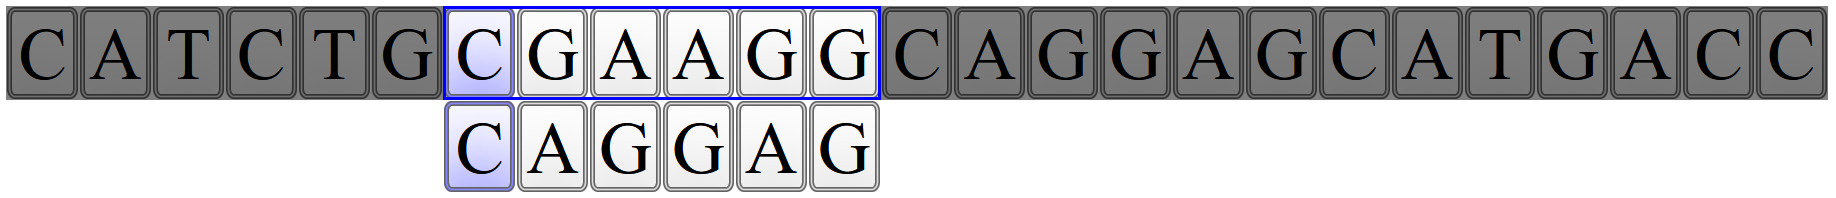
\includegraphics[width=\textwidth]{fenetreglissante4.png}

<< Savoir >> où se situe chaque potentiel mauvais caractère, c'est avoir mémorisé leurs positions dans le motif. On peut le faire dans un pré-traitement du motif.

\begin{définition*}{Tableau des mauvais caractères}
Le tableau des mauvais caractères donne le nombre, strictement positif, de positions à remonter depuis la fin du motif pour trouver chaque caractère possible. Il donne la longueur du motif, si le caractère n'y est pas présent. 
\end{définition*}

\begin{exo} Compléter le tableau des mauvais caractères :

\centering
Motif : {\Large\texttt{CAGGAG}}\qquad \begin{tabular}{|c|c|c|c|}\hline
\rule{0pt}{1.25em}\Large\texttt{A} & \Large\texttt{C} & \Large\texttt{G} & \Large\texttt{T} \\\hline
\rule{0pt}{1.25em}\prof{~~~1}\pointsuite{1cm} & \prof{~~~5}\pointsuite{1cm} & \prof{~~~2}\pointsuite{1cm} & \prof{~~~6}\pointsuite{1cm} \\\hline
\end{tabular}


\end{exo}

\begin{exo} 

\begin{enumerate}
    \item Quelle structure de données est adaptée pour le traitement des mauvais caractères ?
    
    \item Proposer un algorithme donnant le tableau des mauvais caractères, pour un motif et un alphabet donnés.
    
\end{enumerate}

\end{exo}

Correction pour l'exercice \thechapter.\theexo


\begin{algorithm}[H]
\Fct{mauvaisCaractere(motif, alphabet)}{
  $m \leftarrow \text{taille}(\text{motif})$\;
  $\text{mc} \leftarrow $ dictionnaire associant $m$ à chaque lettre de l'alphabet\;
  \Pour{$i$ {\color{black}\bfseries\textrm allant de}  $0$ {\color{black}\bfseries\textrm à} $m-2$}{$\text{mc}[\text{motif}[i]] \leftarrow m-1-i$\;}
  \Retour{mc}
}
\end{algorithm}

\begin{exo} Programmer en Python la fonction proposée ci-dessus.
\end{exo}

\subsection{Algorithme tenant compte du mauvais caractère}

Pour la suite, on notera $i$ l'indice positionnant le début de la fenêtre de recherche sur le texte et $j$ l'indice dans le motif du mauvais caractère s'il y en a un. 

Exemple 1. Ci-dessous : $i=2$ et $j=4$ 

\noindent\begin{tikzpicture}
\clip(0,0)rectangle(\textwidth,1.5em);
\foreach\i in {0,...,24}\node[above=0pt,inner sep = 2pt]at({0.335+\i*0.639},0){\scriptsize\i};
\def\i{2}
\node[above=0pt,inner sep = 2pt, fill=white, circle, draw]at({0.335+\i*0.639},0){$i$};
\end{tikzpicture}
\noindent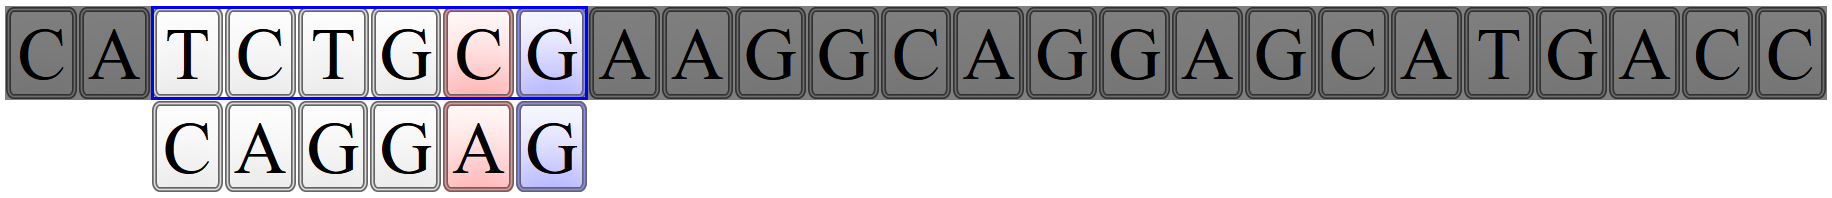
\includegraphics[width=\textwidth]{fenetreglissante5.png}
\noindent\begin{tikzpicture}
\clip(0,0)rectangle(\textwidth,1.5em);
\foreach\j in {0,...,5}\node[below=0pt,inner sep = 2pt]at({0.335+(\j+2)*0.639},1.5em){\scriptsize\j};
\def\j{4}
\node[below=0pt,inner sep = 1pt, fill=white, circle, draw]at({0.335+(\j+2)*0.639},1.5em){$j$};
\end{tikzpicture}


Exemple 2. Ci-dessous : $i=5$ et $j=3$

\noindent\begin{tikzpicture}
\clip(0,0)rectangle(\textwidth,1.5em);
\foreach\i in {0,...,24}\node[above=0pt,inner sep = 2pt]at({0.335+\i*0.639},0){\scriptsize\i};
\def\i{5}
\node[above=0pt,inner sep = 2pt, fill=white, circle, draw]at({0.335+\i*0.639},0){$i$};
\end{tikzpicture}
\noindent
\includegraphics[width=\textwidth]{fenetreglissante2.png}
\noindent\begin{tikzpicture}
\clip(0,0)rectangle(\textwidth,1.5em);
\foreach\j in {0,...,5}\node[below=0pt,inner sep = 2pt]at({0.335+(\j+5)*0.639},1.5em){\scriptsize\j};
\def\j{3}
\node[below=0pt,inner sep = 1pt, fill=white, circle, draw]at({0.335+(\j+5)*0.639},1.5em){$j$};
\end{tikzpicture}


\begin{exo} \addtocounter{exo}{-1}\refstepcounter{exo}\label{algo}Compléter l'algorithme de recherche suivant, prenant en compte les mauvais caractères :

\begin{algorithm}[H]
\Fct{rechercheAvecMC(texte, motif, alphabet)}{
  $\text{mc} \leftarrow $ mauvaisCaractere(motif, alphabet)\;
  $\text{position} \leftarrow  $ liste vide\;
  $i \leftarrow 0$\;     
  \Tq{$i\leqslant\text{taille}(\text{texte})-\text{taille}(\text{motif})$}{
      $j \leftarrow$ \rule{0pt}{1.5em}\prof{taille(motif)$-1$}\pointsuite{3cm}\;      
      \Tq{\rule{0pt}{1.5em}\prof{$j\geqslant0$}\pointsuite{2cm} et $\text{texte}[i+j]=\text{motif}[j]$}
      {   $j \leftarrow $\rule{0pt}{1.5em}\prof{$j-1$}\pointsuite{2cm}\;   }
      \uSi{$j$\prof{$<0$}\pointsuite{2cm}}{
          Ajoute $i$ à position\;
          $i \leftarrow i + 1$\;
      }
      \Sinon{$i \leftarrow i + $ \prof{maximum entre $1$ et $j-\text{taille}(\text{motif})+1+mc[\text{texte}[i+j]]$}\pointsuite{10cm}\;}
  }
  \Retour{position}
}
\end{algorithm}

\end{exo}


\begin{exo} \addtocounter{exo}{-1}\refstepcounter{exo}\label{exemple}En utilisant l'algorithme précédent :

\begin{enumerate}
    \item De combien décale-t-on la fenêtre de l'exemple 1 ? \prof{4}\pointsuite{1cm}
    \item De combien décale-t-on la fenêtre de l'exemple 2 ? \prof{1}\pointsuite{1cm}
    \item De combien décale-t-on la fenêtre s'il n'y a pas de mauvais caractère ? \prof{1}\pointsuite{1cm}
\end{enumerate}

\end{exo}

\begin{exo}Programmer en Python l'algorithme de l'exercice \ref{algo} et vérifier les résultats de l'exercice \ref{exemple}.\end{exo}

\section{Utilisation du bon suffixe}

\subsection{Pré-traitement}

\begin{exo} Cas du bon suffixe redondant

Si le bon suffixe se retrouve dans le motif, précédé d'une lettre différente, on peut en déduire de combien on peut faire glisser la fenêtre. Compléter :

\begin{multicols}{3}\centering

\rule{1.8cm}{0pt}\ding{55}\quad\ding{51}\quad\ding{51}


\includegraphics[height=2.1em]{bonsuffixe3.png}

\medskip On peut décaler de \prof{3}\pointsuite{1cm}

\rule{2.3cm}{0pt}\ding{55}\quad\ding{51}


\includegraphics[height=2.1em]{bonsuffixe4.png}

\medskip On  peut décaler de \prof{2}\pointsuite{1cm}

\rule{2.8cm}{0pt}\ding{55}


\includegraphics[height=2.1em]{bonsuffixe5.png}

\medskip On peut décaler de \prof{1}\pointsuite{1cm}
\end{multicols}
\end{exo}

\begin{exo} Cas du bon suffixe non redondant

Si le bon suffixe ne se retrouve pas dans le motif, précédé d'une lettre différente, alors on  cherche le plus grand suffixe dans le bon suffixe, qui soit aussi un préfixe du motif. S'il n'y en a toujours pas, on peut avancer de la taille du motif.

\begin{multicols}{3}\centering

\rule{1.2cm}{0pt}\ding{55}\quad\ding{51}\quad\ding{51}\quad\ding{51}


\includegraphics[height=2.1em]{bonsuffixea.png}

\medskip On peut décaler de \prof{4}\pointsuite{1cm}

\rule{1.2cm}{0pt}\ding{55}\quad\ding{51}\quad\ding{51}\quad\ding{51}


\includegraphics[height=2.1em]{bonsuffixeb.png}

\medskip On peut décaler de \prof{3}\pointsuite{1cm}

\rule{1.2cm}{0pt}\ding{55}\quad\ding{51}\quad\ding{51}\quad\ding{51}


\includegraphics[height=2.1em]{bonsuffixe2.png}

\medskip On peut décaler de \prof{6}\pointsuite{1cm}

\end{multicols}


\end{exo}

\begin{définition*}{Tableau des bons suffixes}
Pour chaque indice $j$ entre $0$ et $m-1$ donnant la position du mauvais caractère, on appelle << bon suffixe >> la séquence des lettres du motif d'indices strictement supérieurs à $j$.

Le tableau des bons suffixes, donne, pour chaque valeur de $j$, le plus petit déplacement tel que :
\begin{itemize}
    \item un caractère prenant la place d'un caractère du bon suffixe reste << bon >>,
    \item un caractère prenant la place correspondante au mauvais caractère soit différent.
\end{itemize} 
\end{définition*}


\begin{exo} Compléter le tableau des bon suffixes :

\centering
Motif : {\Large\texttt{CAGGAG}}\qquad \begin{tabular}{r|c|c|c|c|c|c|}\cline{2-7}
$j=$&\rule{0pt}{1.25em}\Large\texttt{0} & \Large\texttt{1} & \Large\texttt{2} & \Large\texttt{3} & \Large\texttt{4} & \Large\texttt{5} \\\cline{2-7}
décalage $=$&\rule{0pt}{1.25em}\prof{~~~6}\pointsuite{1cm} & \prof{~~~6}\pointsuite{1cm} & \prof{~~~6}\pointsuite{1cm} & \prof{~~~3}\pointsuite{1cm} & \prof{~~~2}\pointsuite{1cm} & \prof{~~~1}\pointsuite{1cm} \\\cline{2-7}
\end{tabular}


\end{exo}

\begin{exo} Compléter l'algorithme donnant le tableau des bons suffixes :


\begin{algorithm}[H]
\Fct{bonSuffixe(motif)}{
  $\text{m} \leftarrow \text{taille}(\text{motif})$\;
  $\text{bs} \leftarrow  $ tableau de m fois la valeur m\;
  \Pour{$j$ {\color{black}\bfseries\textrm allant de} $0$ {\color{black}\bfseries\textrm à} $\text{m}-1$}{
    décalage $\leftarrow 1$\;     
    \Tq{décalage $<$ \prof{m}\pointsuite{2em} et $\text{bs}[j]=$\prof{m}\pointsuite{2em}}{
      \# k donne les indices correspondants au bon suffixe\;
      $k \leftarrow $ la plus grande valeur entre $j + 1$ et décalage\;     
      \Tq{$k<m$ et \prof{$\text{motif}[k-\text{décalage}]=\text{motif}[k]$}\pointsuite{15em}}{
       $k=k+1$\;
      }
      \Si{$k=m$ et (\prof{$j<$décalage ou $\text{motif}[j-\text{décalage}]\neq \text{motif}[j]$}\pointsuite{25em})}{
        bd$[j] \leftarrow $décalage\;
      }
      décalage $\leftarrow$ décalage $+1$\;
    }
  }
  \Retour{bs}
}
\end{algorithm}

Programmer cet algorithme en Python et vérifier les résultats des exercices précédents.
\end{exo}

\begin{exo} L'algorithme de recherche d'un motif dans un texte, par fenêtre glissante, utilisant les tableaux des mauvais caractères et celui des bons suffixes s'appelle l'algorithme de Boyer–Moore.

Proposer l'écriture de cet algorithme.
\end{exo}

\section{Algorithme de Boyer–Moore}

Résumé des algorithmes pour la recherche Boyer–Moore :

\begin{algorithm}[H]
\Fct{mauvaisCaractere(motif, alphabet)}{
  $m \leftarrow \text{taille}(\text{motif})$\;
  $\text{mc} \leftarrow $ dictionnaire associant $m$ à chaque lettre de l'alphabet\;
  \Pour{$i$ {\color{black}\bfseries\textrm allant de}  $0$ {\color{black}\bfseries\textrm à} $m-2$}{$\text{mc}[\text{motif}[i]] \leftarrow m-1-i$\;}
  \Retour{mc}
}
\end{algorithm}

\begin{algorithm}[H]
\Fct{bonSuffixe(motif)}{
  $\text{m} \leftarrow \text{taille}(\text{motif})$\;
  $\text{bs} \leftarrow  $ tableau de m fois la valeur m\;
  \Pour{$j$ {\color{black}\bfseries\textrm allant de} $0$ {\color{black}\bfseries\textrm à} $\text{m}-1$}{
    décalage $\leftarrow 1$\;     
    \Tq{décalage $<$ m et $\text{bs}[j]=$m}{
      \# k donne les indices correspondants au bon suffixe\;
      $k \leftarrow $ la plus grande valeur entre $j + 1$ et décalage\;   
      \Tq{$k<m$ et $\text{motif}[k-\text{décalage}]=\text{motif}[k]$}{
       $k=k+1$\;
      }
      \Si{$k=m$ et ($j<$décalage ou $\text{motif}[j-\text{décalage}]\neq \text{motif}[j]$)}{
        bd$[j] \leftarrow $décalage\;
      }
      décalage $\leftarrow$ décalage $+1$\;
    }
  }
  \Retour{bs}
}
\end{algorithm}

\begin{algorithm}[H]
\Fct{rechercheBoyerMoore(texte, motif, alphabet)}{
  $\text{mc} \leftarrow $ mauvaisCaractere(motif, alphabet)\;
  $\text{bs} \leftarrow $ bonSuffixe(motif)\;
  $\text{position} \leftarrow  $ liste vide\;
  $i \leftarrow 0$\;     
  \Tq{$i\leqslant\text{taille}(\text{texte})-\text{taille}(\text{motif})$}{
      $j \leftarrow \text{taille}(\text{motif})-1$\;      
      \Tq{$j\geqslant0$ et $\text{texte}[i+j]=\text{motif}[j]$}
      {   $j \leftarrow j-1$\;   }
      \uSi{$j<0$}{
          Ajoute $i$ à position\;
          $i \leftarrow i + \text{bs}[0]$\;
      }
      \Sinon{$i \leftarrow i + $maximum entre $\text{bs}[j]$ et $j-\text{taille}(\text{motif})+1+mc[\text{texte}[i+j]]$\;}
  }
  \Retour{position}
}
\end{algorithm}

\end{document}